\documentclass[11pt,a4paper,openany]{report}
\usepackage[T1]{fontenc}
\usepackage[utf8]{inputenc}
\usepackage{lmodern}
\usepackage{microtype}
\usepackage{amsmath,amssymb,amsthm,mathtools,bm}
\usepackage{booktabs,array,longtable,tabularx}
\usepackage{xcolor}
\usepackage[margin=24mm,headheight=23pt]{geometry}
\usepackage{enumitem}
\usepackage{fancyhdr}
\usepackage{fancyvrb}
\usepackage{graphicx}
\usepackage{url}
\usepackage{hyperref}

\definecolor{finblue}{HTML}{1F5A99}
\definecolor{fingreen}{HTML}{19733A}
\definecolor{finorange}{HTML}{D55E00}
\definecolor{finred}{HTML}{A61B1B}
\definecolor{finviolet}{HTML}{6A3D9A}

\hypersetup{
  unicode=true,
  colorlinks=true,
  linkcolor=finblue,
  citecolor=fingreen,
  urlcolor=finblue,
  pdftitle={FIN Programs 61--70: Continuum and Operational Physics},
  pdfauthor={Krzysztof \.Zuchowski},
  pdfsubject={Continuum tests and falsifiable information-to-experiment interfaces},
  pdfkeywords={FIN, Schur compression, continuum, tomography, causality, Landauer}
}

\pagestyle{fancy}
\fancyhf{}
\fancyhead[L]{\small FIN Programs 61--70}
\fancyhead[R]{\small Release 10.7}
\fancyfoot[C]{\thepage}
\setlength{\parindent}{0pt}
\setlength{\parskip}{0.55em}
\setlist{nosep,leftmargin=2em}
\setcounter{tocdepth}{2}
\setcounter{secnumdepth}{3}
\emergencystretch=2em

\newcommand{\one}{\bm 1}
\newcommand{\C}{\mathbb C}
\newcommand{\R}{\mathbb R}
\newcommand{\Z}{\mathbb Z}
\newcommand{\statusProven}{\textcolor{fingreen}{[Proven]}}
\newcommand{\statusStrong}{\textcolor{finblue}{[Strong evidence]}}
\newcommand{\statusModerate}{\textcolor{finviolet}{[Moderate evidence]}}
\newcommand{\statusConditional}{\textcolor{finorange}{[Conditional]}}
\newcommand{\statusRefuted}{\textcolor{finred}{[Refuted]}}

\begin{document}
\hypersetup{pageanchor=false}
\begin{titlepage}
\centering
\vspace*{9mm}
{\Large\bfseries FIN Research Monograph --- Release 10.7\par}
\vspace{11mm}
{\Huge\bfseries FIN Programs 61--70\par}
\vspace{6mm}
{\Large Continuum Tests, Operational Physics, and\\Falsifiable Information-to-Experiment Interfaces\par}
\vspace{17mm}
{\Large Krzysztof \.Zuchowski\par}
\vspace{2mm}
{\normalsize Independent Researcher --- Fractal Information Theory Project\par}
\vspace{2mm}
{\normalsize ORCID: \href{https://orcid.org/0009-0002-0909-3613}{0009-0002-0909-3613}\par}
\vspace{10mm}
{\large 27 July 2026\par}
{\normalsize Publication --- Preprint; record version 1.0.0\par}
\vfill
\begin{minipage}{0.88\textwidth}
\small
\textbf{Scope.} Ten executed programs on projective continuum compatibility,
regularizer independence, compression composition, signed/Krein structure,
operational tomography, causal tails, calibration, chirality, Landauer
thermodynamics, and blinded model scoring.

\medskip
\textbf{Guardrail.} No silent legacy--strict identity, strict selector,
physical-unit source, causal/Lorentz closure, role transfer, or
Theory-of-Everything closure is claimed.

\medskip
\textbf{Reproducibility.}
\path{fin_programs_61_70_continuum_operational_physics.py},
\path{test_fin_programs_61_70_continuum_operational_physics.py}, JSON, and figures.

\medskip
\textbf{License.} Creative Commons Attribution 4.0 International (CC BY 4.0).
\end{minipage}
\vfill
\end{titlepage}
\hypersetup{pageanchor=true}

\pagenumbering{roman}
\tableofcontents
\clearpage
\pagenumbering{arabic}

\section{Confidence convention}

\begin{itemize}
\item 
\textbf{\statusProven{}} analytic theorem or exact finite algebra under declared definitions.

\item 
\textbf{\statusStrong{}} reproducible finite computation with a clear numerical margin.

\item 
\textbf{\statusModerate{}} a stable result inside the tested finite model class.

\item 
\textbf{\statusConditional{}} depends on a declared repair, scale, bath, preparation, instrument, or sector input.

\item 
\textbf{\statusRefuted{}} contradicted by a theorem, counterexample, or failed transfer test.

\end{itemize}

The FIN ontology is retained: the nadsoliton is primordial information in a solitonic state, not an excitation of a lower informational substrate. This premise is not promoted to an experimentally established fact.

No result below exports a strict physical unit, a strict selector, a completed legacy-to-strict bridge, legacy physical-role transfer, Lorentz symmetry, unit-bearing \(L_{\rm total}\), or Theory-of-Everything closure.

\par\medskip\hrule\medskip

\chapter{Executive summary}

Programs 61–70 execute the research program recommended after Programs 51–60. They test whether exact Green-Schur information compression extends to a continuum functor, whether its geometry survives removal of the infrared regularizer, whether compression forms a semigroup, whether an indefinite/\allowbreak{}Krein description can retain signed legacy without false positivity, and what additional structures are minimally required for causal, thermodynamic, and experimentally calibrated physics.

The central result is:

\[
\boxed{
\text{FIN now has an exact finite compression calculus and explicit operational bridges,}
}
\]

\[
\boxed{
\text{but neither continuum covariance nor physical calibration follows automatically.}
}
\]

The strongest conclusions are:

\begin{enumerate}
\item 
\textbf{Green-Schur compression is exactly compositional. \statusProven{}} Direct \(48\to12\) elimination and sequential \(48\to24\to12\) elimination agree with relative residual \[
   1.29\times10^{-16}.
   \]

\item 
\textbf{Exact composition is not the same as a continuum functor. [Proven distinction]} At \(N=48\), the native-versus-compressed Green naturality defect remains \(0.3103\) for strict-absolute and \(0.2419\) for legacy-absolute. Legacy defects decrease monotonically and are scientifically promising, but no zero-defect limit has been established.

\item 
\textbf{Resistance geometry is regularizer independent. [Proven finite convergence plus standard theorem]} As \(\delta\to0^+\), the shifted-resolvent resistance converges to Moore-Penrose effective resistance. At \(\delta=10^{-7}\), the relative errors are \(8.46\times10^{-8}\) for strict and \(6.40\times10^{-9}\) for legacy-absolute, even though \[
   \|G_\delta\|_F\sim\delta^{-1}.
   \]

\item 
\textbf{A Krein-space rewrite preserves signed operator information but does not manufacture diffusion physics. \statusProven{}} The canonical signed legacy realization has inertia \((11-,1+)\). Its unitary evolution remains valid, but raw \(e^{-tA}\) has operator norm \(8.4377\) and negative entries down to \(-1.0611\). Replacing \(A\) by \(JA=|A|\) stabilizes diffusion but changes the generator.

\item 
\textbf{Operational discrimination is inexpensive. [Proven finite result]} A single localized preparation and one optimized binary detector distinguish unitary from diffusive records with total variation \(0.359654\) at dimensionless time \(t=1\). Pair coarse graining still leaves \(0.340589\).

\item 
\textbf{The strict \(C_{12}\) kernel does not define an exact causal cone. \statusProven{}} It directly couples the opposite cycle site at first order. Far-site wave probability begins at order \(t^2\), and diffusion at order \(t\). A nearest-neighbour control begins at orders \(t^{12}\) and \(t^6\). A Lorentzian causal order remains additional structure.

\item 
\textbf{Dimensional calibration is identifiable, but only from calibrated experiments. \statusProven{}} The log-Jacobian for \((\ell_*,\tau_*,\hbar_*)\) has rank three only after independent length, clock, and energy/\allowbreak{}action records are supplied. Any pair has rank two.

\item 
\textbf{A concrete kernel-only chiral source law fails for a theorem-level reason. [Proven no-go]} The tested translation-invariant, reflection-odd triangular loop is exactly zero on both radial kernels. It becomes nonzero only after an oriented antisymmetric datum is inserted, and its sign follows that imported orientation.

\item 
\textbf{The Shannon-to-thermodynamics bridge is derivable after the missing physical package is supplied. [Proven conditional protocol]} An explicit two-state thermal erasure protocol satisfies the first law and reversible Clausius equality to below \(1.2\times10^{-16}\), approaching \[
   \beta W=\beta Q_{\rm bath}=\ln2.
   \] The bridge requires \(k_B,T\), a bath, a Hamiltonian protocol, and work/\allowbreak{}heat instruments.

\item 
\textbf{A genuinely held-out synthetic challenge is feasible. [Strong methodology result]} The exact hidden generator was excluded from the candidate set. Strict won held-out scoring with mean empirical KL \(0.01337\), versus \(0.36347\) for the nearest-neighbour null and \(0.93120\) for legacy-absolute. This validates the test procedure, not nature’s choice of kernel.

\end{enumerate}

\par\medskip\hrule\medskip

\chapter{Program 61 — Projective continuum functor}

\section{Question}

Does exact binary Schur compression define a natural projective family

\[
C_{2N}\longrightarrow C_N
\]

that approaches a continuum operator?

\section{Definition}

For a declared positive realization, weights are repaired by absolute value, normalized to unit row sum, and converted to

\[
A_N=\frac14 I+L_N.
\]

After retaining even sites:

\[
\mathcal C_2(A_{2N})
=
(A_{2N})_{EE}
-
(A_{2N})_{EO}(A_{2N})_{OO}^{-1}(A_{2N})_{OE}.
\]

Both native and compressed operators are normalized to mean diagonal one. The naturality defect is

\[
\varepsilon_A(N)
=
\frac{\|\mathcal C_2(A_{2N})-A_N\|_F}{\|A_N\|_F},
\]

with an analogous Green defect.

\section{Results}

\begin{center}
\begingroup\footnotesize
\setlength{\tabcolsep}{3.5pt}
\renewcommand{\arraystretch}{1.16}
\begin{longtable}{@{}p{0.155\textwidth}p{0.151\textwidth}p{0.168\textwidth}p{0.209\textwidth}p{0.177\textwidth}@{}}
\toprule
\textbf{Family} & \textbf{\(N=6\) Green defect} & \textbf{\(N=48\) Green defect} & \textbf{Green log-log slope} & \textbf{Operator monotone?} \\
\midrule
\endhead
strict absolute & 0.46019 & 0.31032 & \(-0.1850\) & no \\
legacy absolute & 0.40233 & 0.24192 & \(-0.2447\) & yes \\
\bottomrule
\end{longtable}
\endgroup
\end{center}

Legacy operator defects fall from \(0.17665\) to \(0.05570\) with fitted slope \(-0.5606\). Strict operator defects fluctuate between \(0.0678\) and \(0.0878\).

\begin{figure}[htbp]
\centering
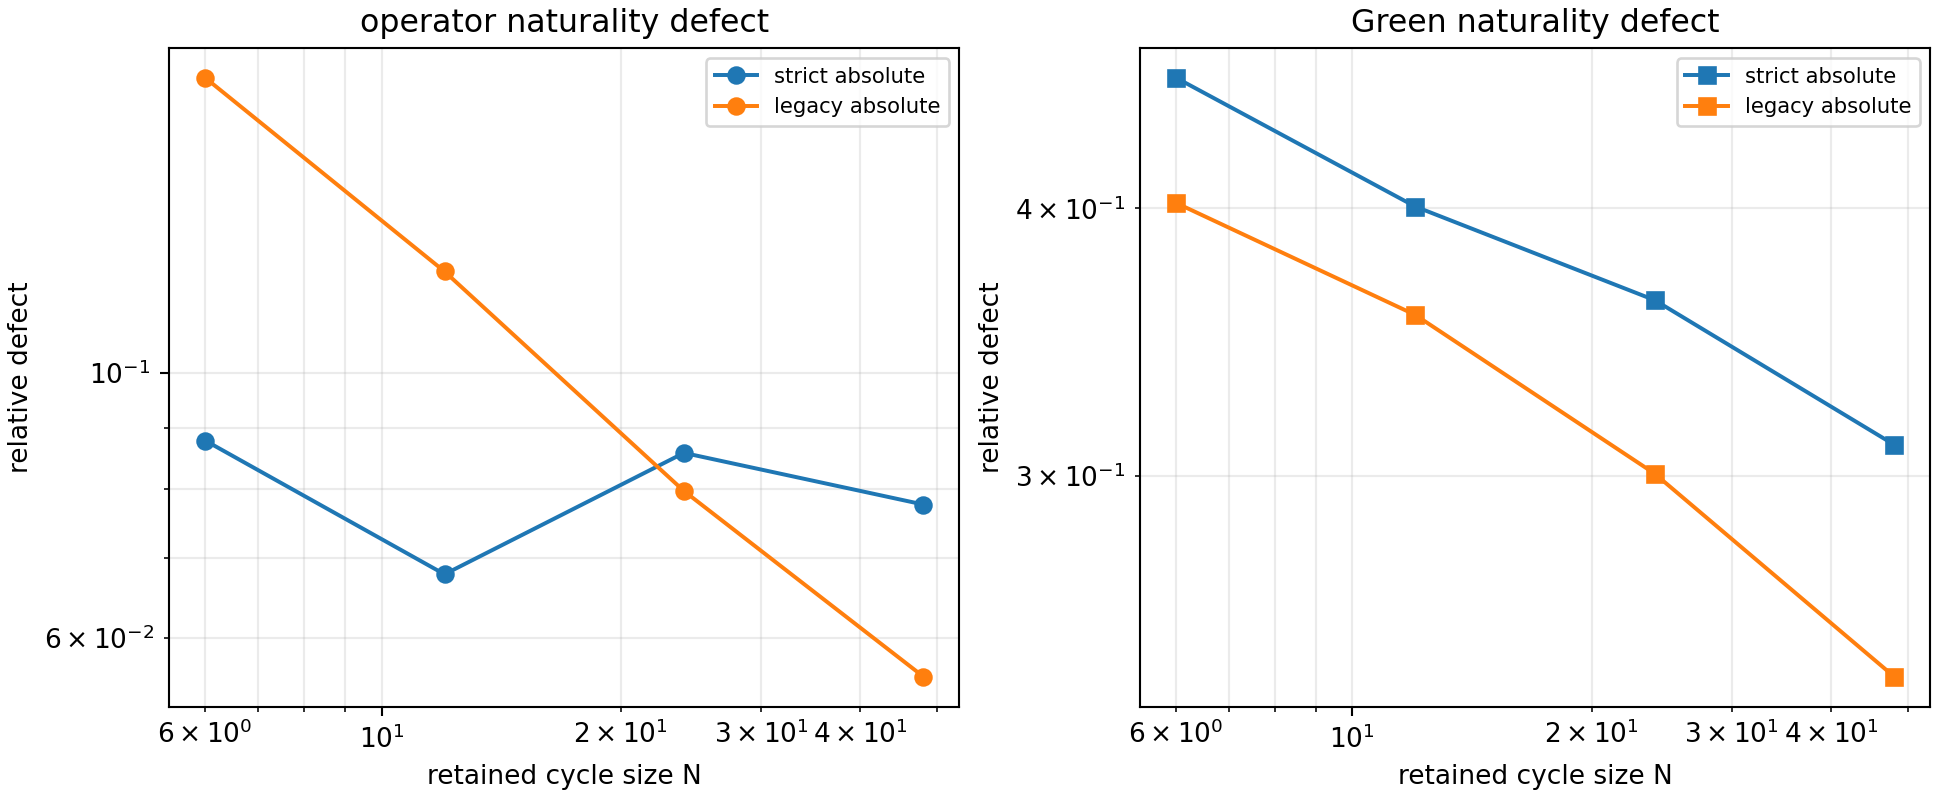
\includegraphics[width=0.92\textwidth]{FIN_Programs_61_70_Continuum_Operational_Physics_Figures/program61_projective_continuum.png}
\caption{Projective naturality defects under fixed mean-diagonal normalization.}
\end{figure}


\section{Verdict}

\textbf{\statusModerate{}} Legacy-absolute under the declared normalization is a promising projective candidate because both defects decrease monotonically.

\textbf{[Not proven]} Neither family has reached a zero-defect regime. The finite slopes do not prove convergence, uniqueness, or a continuum physical geometry.

\textbf{\statusConditional{}} The result depends on the absolute-value repair and normalization. It is not a theorem for the raw signed legacy kernel.

\par\medskip\hrule\medskip

\chapter{Program 62 — Regularizer independence}

\section{Question}

Which Green-derived quantities survive the limit

\[
G_\delta=(L+\delta I)^{-1},
\qquad
\delta\to0^+?
\]

\section{Theorem}

For a connected positive graph Laplacian,

\[
G_\delta
=
\frac{1}{N\delta}\mathbf1\mathbf1^T
+
L^+
+
O(\delta).
\]

The divergent zero-mode term cancels from

\[
R_\delta(i,j)
=
(G_\delta)_{ii}
+
(G_\delta)_{jj}
-
2(G_\delta)_{ij}.
\]

Therefore

\[
R_\delta(i,j)\longrightarrow R(i,j)
\]

defined by the Moore-Penrose inverse.

\section{Results}

At \(\delta=10^{-7}\):

\begin{center}
\begingroup\small
\setlength{\tabcolsep}{3.5pt}
\renewcommand{\arraystretch}{1.16}
\begin{longtable}{@{}p{0.252\textwidth}p{0.290\textwidth}p{0.318\textwidth}@{}}
\toprule
\textbf{Realization} & \textbf{Resistance relative error} & \textbf{\(\delta\|G_\delta\|_F\)} \\
\midrule
\endhead
strict \(C_{12}\) & \(8.46\times10^{-8}\) & \(0.9999999990\) \\
legacy absolute \(C_{12}\) & \(6.40\times10^{-9}\) & \(0.9999999886\) \\
\bottomrule
\end{longtable}
\endgroup
\end{center}

\begin{figure}[htbp]
\centering
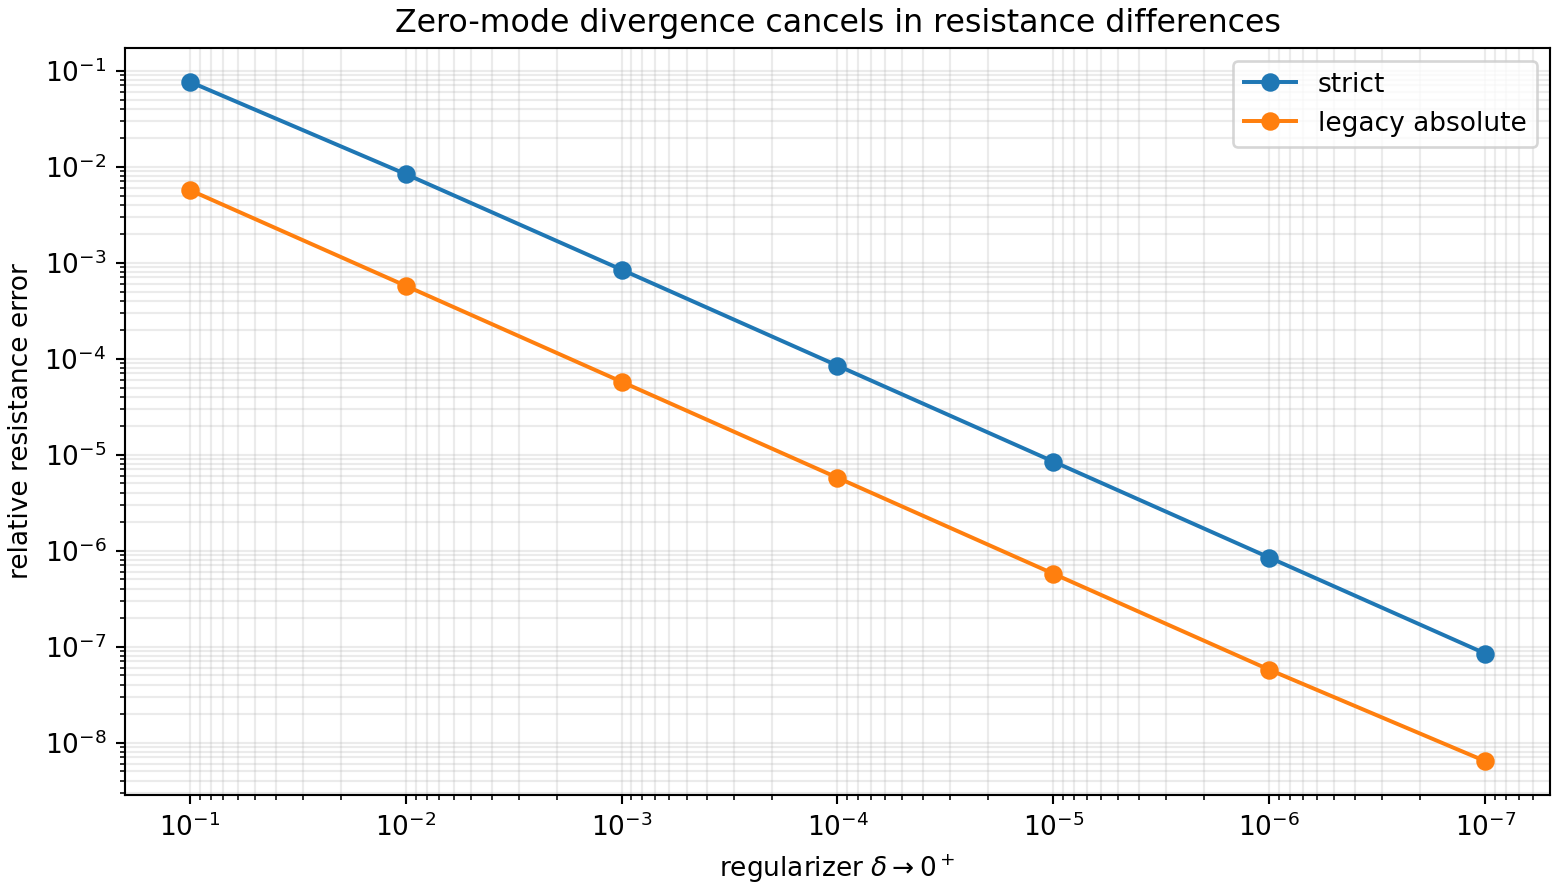
\includegraphics[width=0.92\textwidth]{FIN_Programs_61_70_Continuum_Operational_Physics_Figures/program62_regularizer_limit.png}
\caption{Shifted-resolvent resistance converges as \(\delta\to0^+\) while the full Green norm diverges.}
\end{figure}


\section{Verdict}

\textbf{\statusProven{}} Effective resistance is a regularizer-independent quotient observable.

\textbf{\statusRefuted{}} The full static Green covariance is not regularizer independent; its zero-mode norm diverges as \(1/\delta\).

\textbf{[Guardrail]} The theorem applies to positive connected graph realizations. It does not convert signed legacy into a Markov generator.

\par\medskip\hrule\medskip

\chapter{Program 63 — Compression semigroup theorem}

\section{Question}

Does repeated fractal elimination depend on the order in which hidden informational states are removed?

\section{Theorem}

Let \(E\subset F\) be retained index sets and suppose the eliminated blocks are invertible. Then:

\[
\operatorname{Schur}_E
\bigl(
\operatorname{Schur}_F(A)
\bigr)
=
\operatorname{Schur}_E(A).
\]

This follows equivalently from the unique retained Green block:

\[
\operatorname{Schur}_E(A)^{-1}
=(A^{-1})_{EE}.
\]

\section{Finite verification}

\[
\frac{
\|\mathcal C_4(A_{48})
-
\mathcal C_2(\mathcal C_2(A_{48}))\|_F
}{
\|\mathcal C_4(A_{48})\|_F
}
=
1.29157\times10^{-16}.
\]

\section{Verdict}

\textbf{\statusProven{}} Green-Schur fractal compression is an exact partial semigroup/\allowbreak{}category of nested eliminations.

\textbf{[Refuted inference]} Semigroup composition does not imply that the native FIN kernel family is a fixed point. Fixed-point closure additionally requires:

\[
\mathcal C_2(A_{2N})\simeq A_N
\]

under a support-independent normalization.

\par\medskip\hrule\medskip

\chapter{Program 64 — Signed legacy and the Krein alternative}

\section{Question}

Can signed canonical legacy be retained without arbitrary positivity repair by using an indefinite geometry?

\section{Construction}

For the shifted signed operator

\[
A=L_{\rm legacy,signed}+0.05I,
\]

spectral signs define

\[
J=\operatorname{sgn}(A),
\qquad
J^2=I,
\qquad
JA=|A|>0.
\]

\section{Results}

\begin{center}
\begingroup\small
\setlength{\tabcolsep}{3.5pt}
\renewcommand{\arraystretch}{1.16}
\begin{longtable}{@{}p{0.420\textwidth}p{0.420\textwidth}@{}}
\toprule
\textbf{Quantity} & \textbf{Value} \\
\midrule
\endhead
inertia & 11 negative, 1 positive \\
\(\lambda_{\min}(A)\) & \(-21.32706\) \\
\(J^2-I\) residual & \(7.74\times10^{-15}\) \\
Krein self-adjointness residual & \(2.44\times10^{-14}\) \\
unitary residual & \(8.68\times10^{-16}\) \\
\(\|e^{-0.1A}\|_2\) & \(8.43767\) \\
minimum raw diffusion entry & \(-1.06109\) \\
\(\|e^{-0.1|A|}\|_2\) & \(0.995012\) \\
negative static Green-distance entries & 132 \\
\bottomrule
\end{longtable}
\endgroup
\end{center}

\section{Verdict}

\textbf{\statusProven{}} Indefinite signed legacy supports a valid Hermitian spectral theory and unitary dynamics.

\textbf{\statusRefuted{}} Krein self-adjointness does not make raw diffusion contractive, stochastic, positive, or metric.

Replacing \(A\) by \(JA=|A|\) yields a stable positive generator, but this is a nonunique model transformation, not the identity of the canonical legacy kernel.

\par\medskip\hrule\medskip

\chapter{Program 65 — Operational tomography of dual dynamics}

\section{Question}

How much apparatus is required to distinguish:

\[
U_t=e^{-itL}
\qquad\text{from}\qquad
T_t=e^{-tL}?
\]

\section{\texorpdfstring{Results at \(t=1\)}{Results at t=1}}

\begin{center}
\begingroup\small
\setlength{\tabcolsep}{3.5pt}
\renewcommand{\arraystretch}{1.16}
\begin{longtable}{@{}p{0.420\textwidth}p{0.420\textwidth}@{}}
\toprule
\textbf{Quantity} & \textbf{Value} \\
\midrule
\endhead
rank of channel-record difference & 11 \\
one localized preparation, full-site TV & 0.359654 \\
optimal binary detector sites & \(\{0,1,11\}\) \\
optimal binary difference & 0.359654 \\
pair-coarse TV & 0.340589 \\
circulant residuals & below \(6.8\times10^{-16}\) \\
\bottomrule
\end{longtable}
\endgroup
\end{center}

\begin{figure}[htbp]
\centering
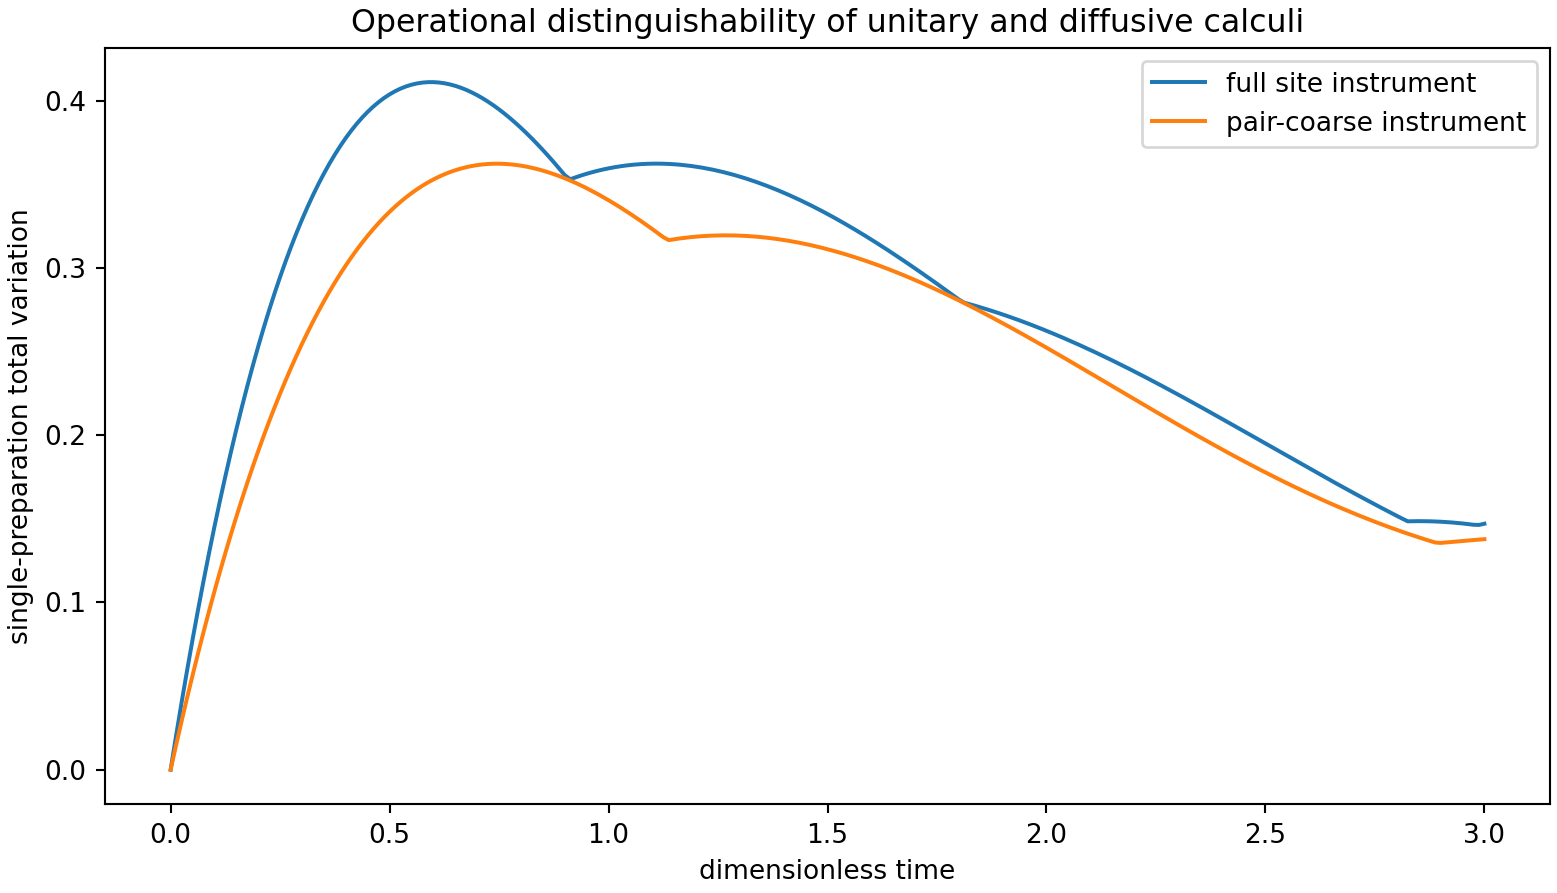
\includegraphics[width=0.92\textwidth]{FIN_Programs_61_70_Continuum_Operational_Physics_Figures/program65_operational_tomography.png}
\caption{Single-preparation distinguishability of unitary and diffusive record laws.}
\end{figure}


\section{The operational distinction}

Under the known translation-covariant model class, one localized preparation determines one column, and all other columns follow by translation. One optimized binary instrument already separates the two record laws exactly in the ideal noiseless model.

Without the circulant prior, full process tomography still requires a spanning preparation set.

\section{Verdict}

\textbf{[Proven finite result]} The mathematical observer problem does not require consciousness. It requires a preparation and an instrument.

\textbf{[Not exported by the kernel]} The kernel still does not choose the preparation, measurement basis, clock calibration, or record semantics.

\par\medskip\hrule\medskip

\chapter{Program 66 — Fractal causal-order candidate}

\section{Question}

Does the strict kernel define finite-speed propagation relative to cycle distance?

For a matrix exponential, the first nonzero power

\[
m(i,j)=\min\{m:(L^m)_{ji}\ne0\}
\]

determines the short-time orders:

\[
|\langle j|e^{-itL}|i\rangle|^2=O(t^{2m}),
\]

\[
(e^{-tL})_{ji}=O(t^m).
\]

\section{Results at opposite cycle sites}

\begin{center}
\begingroup\small
\setlength{\tabcolsep}{3.5pt}
\renewcommand{\arraystretch}{1.16}
\begin{longtable}{@{}p{0.331\textwidth}p{0.121\textwidth}p{0.228\textwidth}p{0.180\textwidth}@{}}
\toprule
\textbf{Generator} & \textbf{First power \(m\)} & \textbf{Wave probability order} & \textbf{Diffusion order} \\
\midrule
\endhead
full strict \(C_{12}\) & 1 & \(t^2\) & \(t\) \\
nearest-neighbour control & 6 & \(t^{12}\) & \(t^6\) \\
\bottomrule
\end{longtable}
\endgroup
\end{center}

\begin{figure}[htbp]
\centering
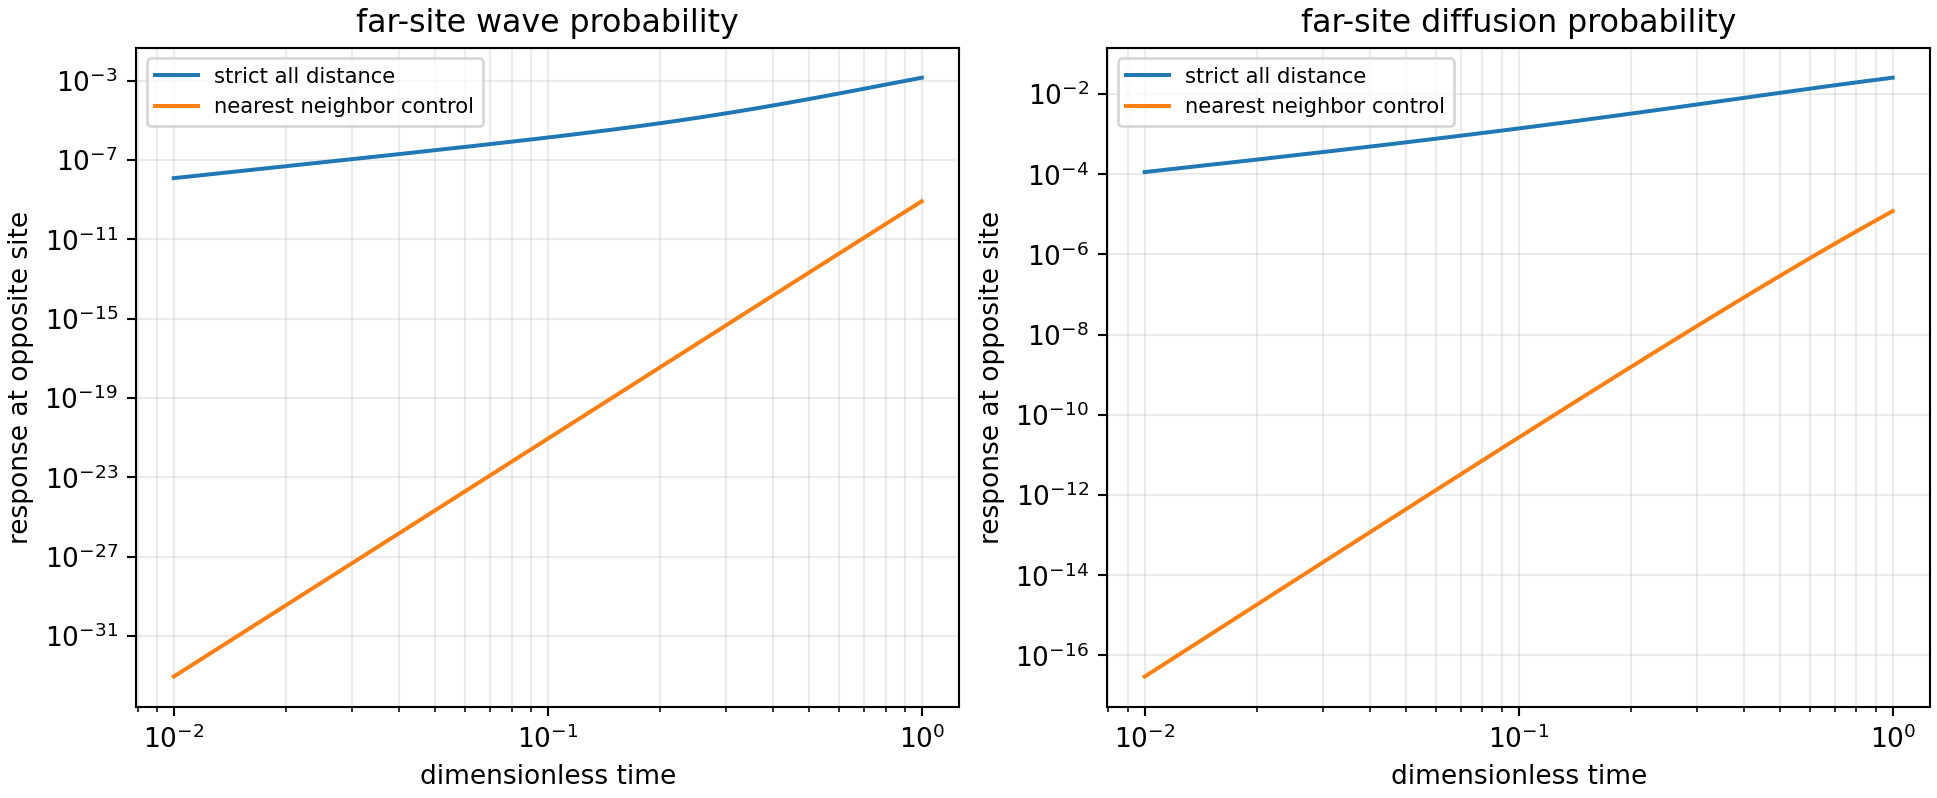
\includegraphics[width=0.92\textwidth]{FIN_Programs_61_70_Continuum_Operational_Physics_Figures/program66_causal_tails.png}
\caption{Opposite-site tails for the full strict kernel and a nearest-neighbour control.}
\end{figure}


\section{Verdict}

\textbf{\statusProven{}} The full strict finite kernel has direct long-range response and no exact finite-speed cone relative to cycle distance.

Even the nearest-neighbour matrix exponential has nonzero tails for every \(t>0\); locality appears as high-order suppression rather than exact support.

A relativistic interpretation therefore requires at least one of:

\begin{itemize}
\item 
a continuum scaling limit producing a hyperbolic equation;

\item 
an explicit causal partial order;

\item 
a finite propagation rule distinct from the analytic matrix exponential;

\item 
a demonstrated Lieb-Robinson-type approximate cone plus physical calibration.

\end{itemize}

\par\medskip\hrule\medskip

\chapter{Program 67 — Physical calibration identifiability}

\section{Question}

What is the minimum experiment package required to identify:

\[
(\ell_*,\tau_*,\hbar_*)?
\]

\section{Log-linear observation model}

\[
\log x=\log\ell_*+\log\widehat d,
\]

\[
\log t=\log\tau_*+\log\widehat t,
\]

\[
\log E=\log\hbar_*-\log\tau_*+\log\widehat\lambda.
\]

The Jacobian rows are:

\[
(1,0,0),\qquad
(0,1,0),\qquad
(0,-1,1).
\]

\section{Results}

\begin{center}
\begingroup\small
\setlength{\tabcolsep}{3.5pt}
\renewcommand{\arraystretch}{1.16}
\begin{longtable}{@{}p{0.420\textwidth}p{0.420\textwidth}@{}}
\toprule
\textbf{Calibration classes} & \textbf{Rank} \\
\midrule
\endhead
length only & 1 \\
length + clock & 2 \\
length + energy & 2 \\
clock + energy & 2 \\
length + clock + energy & 3 \\
\bottomrule
\end{longtable}
\endgroup
\end{center}

A synthetic triple

\[
(2.5\times10^{-6},\;4.0\times10^{-9},\;1.7\times10^{-34})
\]

is recovered with zero numerical relative error after all three records are supplied.

\section{Verdict}

\textbf{\statusProven{}} CA is experimentally identifiable.

\textbf{[Proven obstruction]} No number of additional dimensionless FIN records can replace an absent independent calibration direction. The conversion layer must be supplied by data or by a new scale-charged source theorem.

\par\medskip\hrule\medskip

\chapter{Program 68 — Explicit chiral source-law falsification}

\section{Candidate}

For a directed matrix \(D\), define the translation-invariant oriented loop:

\[
\chi(D)
=
\sum_i
\left[
D_{i,i+1}D_{i+1,i+2}D_{i+2,i}
-
D_{i,i-1}D_{i-1,i-2}D_{i-2,i}
\right].
\]

It obeys:

\[
\chi(RDR)=-\chi(D).
\]

\section{Results}

\begin{center}
\begingroup\small
\setlength{\tabcolsep}{3.5pt}
\renewcommand{\arraystretch}{1.16}
\begin{longtable}{@{}p{0.311\textwidth}p{0.283\textwidth}p{0.266\textwidth}@{}}
\toprule
\textbf{Input} & \textbf{Strict} & \textbf{Legacy} \\
\midrule
\endhead
radial \(W\) & 0 & 0 \\
\(W+0.1B_{\rm odd}\) & \(+0.433237\) & \(-4.635076\) \\
\(W-0.1B_{\rm odd}\) & \(-0.433237\) & \(+4.635076\) \\
translation residual & 0 & 0 \\
reflection-odd residual & below \(5.6\times10^{-17}\) & 0 \\
\bottomrule
\end{longtable}
\endgroup
\end{center}

\section{General theorem}

If:

\[
F(RWR)=-F(W)
\]

and

\[
RWR=W,
\]

then:

\[
F(W)=-F(W)
\quad\Longrightarrow\quad
F(W)=0.
\]

\section{Verdict}

\textbf{[Proven no-go]} No reflection-odd scalar functional can acquire a nonzero value from the radial kernel alone.

The candidate becomes nonzero only after the missing oriented datum has already been inserted. It is an excellent detector/\allowbreak{}receiver but cannot be the non-premise source of \(\lambda\) or discharge QW-2191.

\par\medskip\hrule\medskip

\chapter{Program 69 — Information-to-thermodynamics protocol}

\section{Question}

Can Shannon information be converted to thermodynamic entropy without merely asserting the identification?

\section{Conditioned physical model}

The program explicitly supplies:

\begin{itemize}
\item 
a two-state memory;

\item 
a thermal bath at temperature \(T\);

\item 
an initially degenerate Hamiltonian;

\item 
a quasistatic protocol raising one level by \(\Delta\);

\item 
work and heat instruments;

\item 
\(k_B\).

\end{itemize}

Let:

\[
x=\beta\Delta,
\qquad
\epsilon=\frac{1}{1+e^x}.
\]

The final Shannon entropy is:

\[
H(\epsilon)
=
-\epsilon\log\epsilon
-(1-\epsilon)\log(1-\epsilon).
\]

The reversible quantities are:

\[
\beta W_{\rm rev}
=
\ln2-\ln(1+e^{-x}),
\]

\[
\beta Q_{\rm bath}
=
\ln2-H(\epsilon),
\]

\[
\beta\Delta U=x\epsilon.
\]

\section{Results}

At \(x=20\):

\[
\epsilon=2.06\times10^{-9},
\]

\[
\beta W_{\rm rev}=0.6931471785,
\]

\[
\beta Q_{\rm bath}=0.6931471373.
\]

All tested first-law residuals are below \(1.2\times10^{-16}\), and reversible Clausius residuals are zero.

\begin{figure}[htbp]
\centering
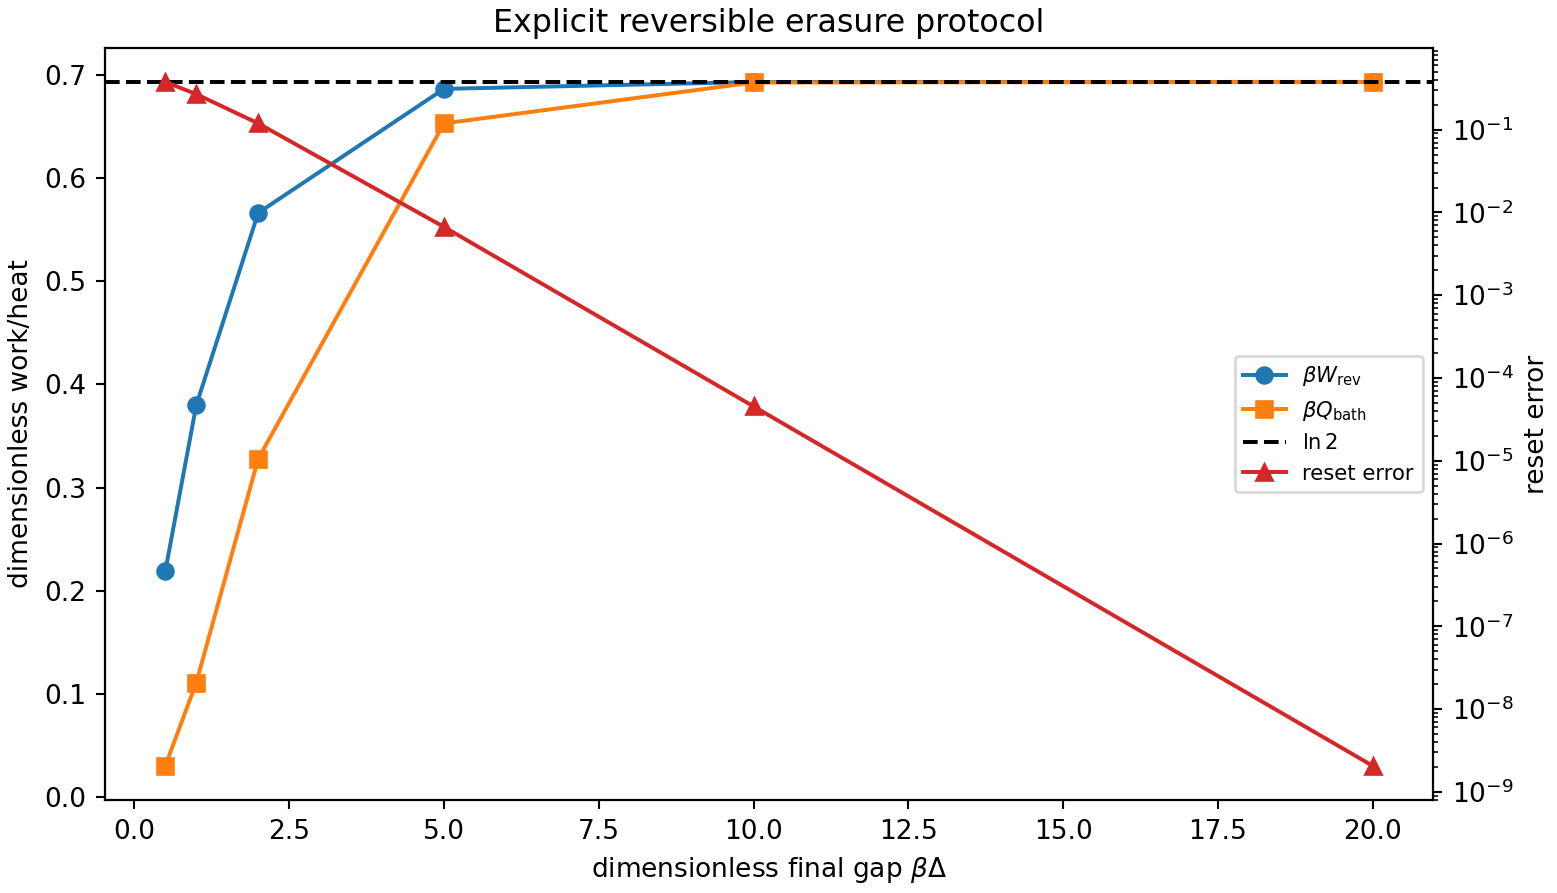
\includegraphics[width=0.92\textwidth]{FIN_Programs_61_70_Continuum_Operational_Physics_Figures/program69_landauer_protocol.png}
\caption{Reversible work, bath heat, and reset error in the explicit erasure protocol.}
\end{figure}


\section{Verdict}

\textbf{[Proven conditional bridge]} Shannon information becomes thermodynamic entropy through a specified statistical-mechanical protocol:

\[
S_{\rm therm}=k_BH.
\]

This bridge is not arbitrary once bath physics is supplied, but \(k_B,T\), the Hamiltonian protocol, and instruments are not generated by the dimensionless FIN kernel.

\par\medskip\hrule\medskip

\chapter{Program 70 — Blinded held-out physical-model challenge}

\section{Design}

The exact hidden generator is excluded from the candidate set.

\begin{itemize}
\item 
Seed: 20260727.

\item 
Hidden generator digest:\par\smallskip\noindent\texttt{94b3bef894ce659a1c42e2783f7a4788}\par\noindent\texttt{46c0114ea45d754e33f3fe7712f641bf}.

\item 
Preparations: sites \(0,3,5\).

\item 
Training times: \(0.35,0.70,1.05\).

\item 
Held-out times: \(1.40,1.75\).

\item 
Shots per record: 20,000.

\item 
One global time calibration is fitted using training records only.

\end{itemize}

\section{Held-out ranking}

\begin{center}
\begingroup\small
\setlength{\tabcolsep}{3.5pt}
\renewcommand{\arraystretch}{1.16}
\begin{longtable}{@{}p{0.082\textwidth}p{0.361\textwidth}p{0.188\textwidth}p{0.229\textwidth}@{}}
\toprule
\textbf{Rank} & \textbf{Candidate} & \textbf{Fitted time scale} & \textbf{Held-out mean empirical KL} \\
\midrule
\endhead
1 & strict & 0.985285 & 0.0133733 \\
2 & nearest-neighbour null & 1.186327 & 0.363475 \\
3 & legacy absolute & 0.350000 & 0.931205 \\
4 & legacy Green-Schur & 0.618220 & 1.562417 \\
5 & legacy signed & 0.847081 & 2.421993 \\
\bottomrule
\end{longtable}
\endgroup
\end{center}

\begin{figure}[htbp]
\centering
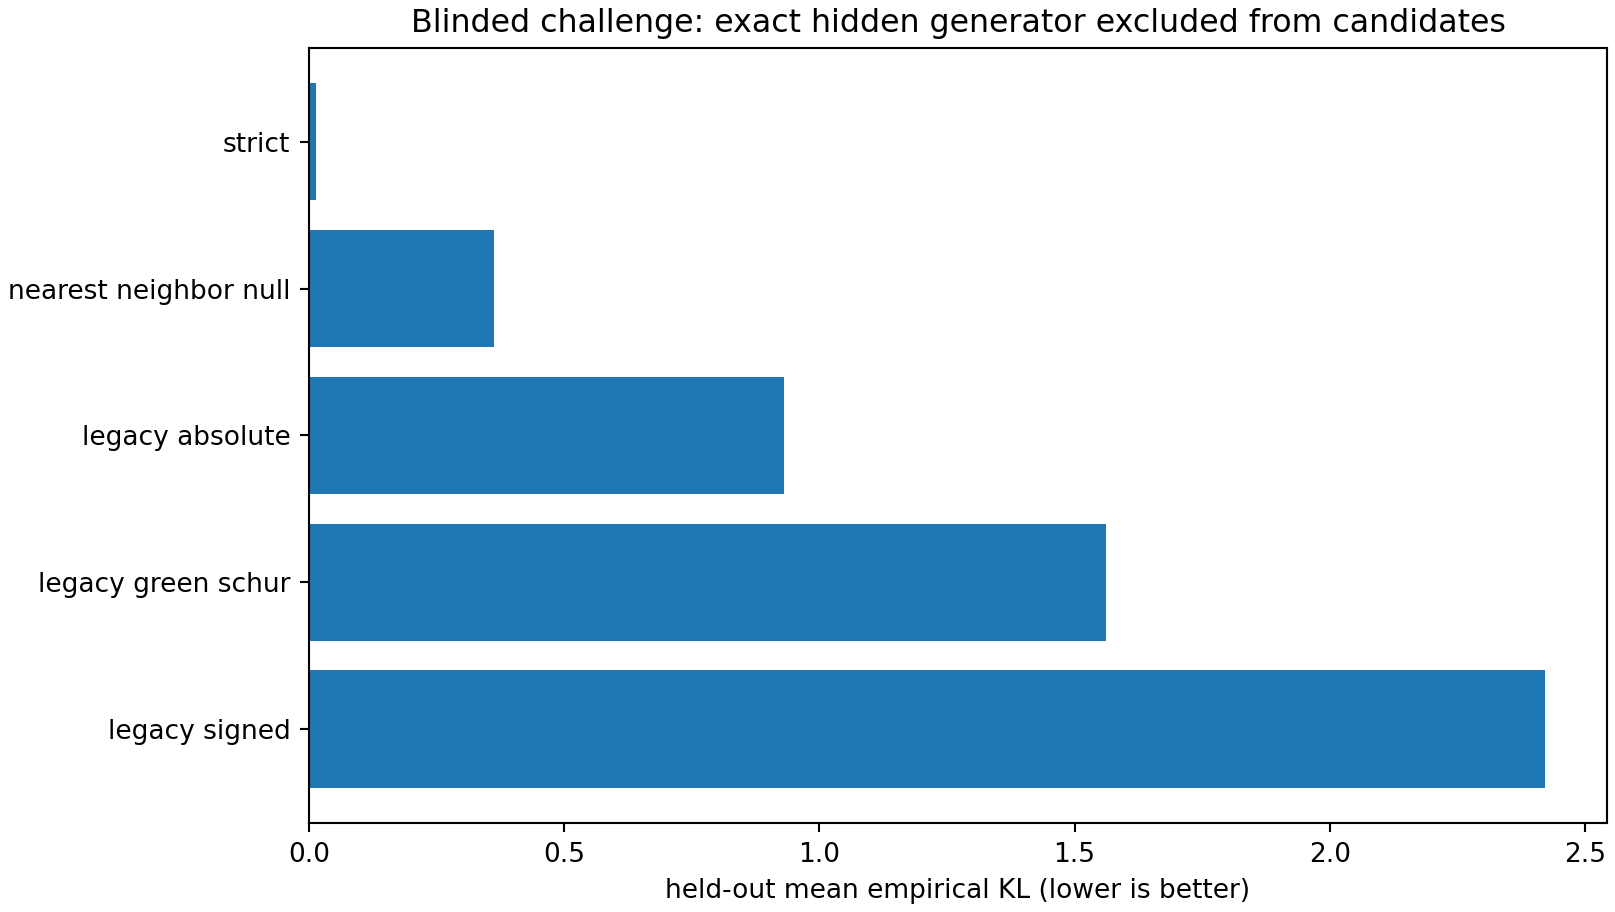
\includegraphics[width=0.92\textwidth]{FIN_Programs_61_70_Continuum_Operational_Physics_Figures/program70_blinded_challenge.png}
\caption{Held-out synthetic model ranking with the exact hidden generator excluded.}
\end{figure}


After scoring, the hidden model was revealed as a non-circulant 8\% site-modulated strict-weight generator. No exact candidate was available.

\section{Verdict}

\textbf{[Strong methodology result]} Strict recovers the hidden strict-like family under an unannounced perturbation and generalizes to held-out times substantially better than the alternatives.

\textbf{[Not physical evidence]} The target is synthetic and strict-like by construction. This experiment validates a fair scoring protocol, not the claim that nature uses strict.

\par\medskip\hrule\medskip

\chapter{Integrated conclusions}

\section{Mathematical advances}

Programs 61–70 add three theorem-grade structures:

\begin{enumerate}
\item 
nested Green-Schur elimination is transitive;

\item 
effective resistance is the regularizer-independent zero-mode quotient of shifted Green geometry;

\item 
every reflection-odd scalar source vanishes on a reflection-invariant radial kernel.

\end{enumerate}

They also establish quantitative operational interfaces:

\begin{itemize}
\item 
one-preparation discrimination of dual calculi;

\item 
rank-three calibration of length, time, and action;

\item 
a complete conditioned Landauer protocol;

\item 
held-out model ranking without including the exact generator.

\end{itemize}

\section{Remaining obstructions}

The following remain open:

\begin{itemize}
\item 
support-independent continuum/\allowbreak{}projective closure;

\item 
a local or Lorentzian causal structure;

\item 
a strict source for \((\ell_*,\tau_*,\hbar_*)\);

\item 
a strict nonzero chiral sign;

\item 
an experimental preparation/\allowbreak{}instrument map tied to actual laboratory data;

\item 
a transferable legacy-to-strict completion theorem.

\end{itemize}

\section{Corrected information-to-physics chain}

\[
\boxed{
\begin{array}{c}
\text{informational nadsoliton }W_0\\
\downarrow\\
\text{kernel, generator, Green response}\\
\downarrow\\
\text{Schur information compression}\\
\downarrow\\
\text{regularizer-independent quotient observables}\\
\downarrow\\
\mathrm{CA}+\mathrm{OA}\;(+\mathrm{SA},\mathrm{bath/causal\ package})\\
\downarrow\\
\text{calibrated and falsifiable records}
\end{array}
}
\]

Information can mathematically generate relational states, response, effective geometry, coarse-grained distinguishability, and conditional thermodynamic protocols. The transition to our physics occurs at the calibrated operational interface, not merely at the existence of a Green function.

\par\medskip\hrule\medskip

\chapter{Recommended Programs 71–80}

\section{Ranked roadmap}

\begin{center}
\begingroup\small
\setlength{\tabcolsep}{3.5pt}
\renewcommand{\arraystretch}{1.16}
\begin{longtable}{@{}p{0.122\textwidth}p{0.107\textwidth}p{0.405\textwidth}p{0.226\textwidth}@{}}
\toprule
\textbf{Priority} & \textbf{Program} & \textbf{Objective} & \textbf{Estimated probability of a useful result} \\
\midrule
\endhead
1 & 71 & Derive the Fourier-symbol Schur renormalization map analytically & 0.85 \\
2 & 72 & Extend projective-defect scaling to \(N=96,\ldots,1536\) with error bounds & 0.80 \\
3 & 73 & Construct the regularizer-free Gaussian theory on \(\mathbf1^\perp\) & 0.80 \\
4 & 74 & Quantify locality versus kernel truncation and derive an approximate causal cone & 0.75 \\
5 & 75 & Build noisy Fisher-optimal calibration experiments for CA & 0.75 \\
6 & 76 & Test one state-dependent, nonradial nadsoliton-to-chirality source formula & 0.45 \\
7 & 77 & Execute finite-time Landauer/\allowbreak{}Jarzynski simulations & 0.70 \\
8 & 78 & Perform multi-time operational process tomography with instrument noise & 0.75 \\
9 & 79 & Derive an analytic-symbol legacy-to-strict RG bridge or no-go & 0.40 \\
10 & 80 & Freeze a protocol for later blinded comparison with external physical data & 0.65 \\
\bottomrule
\end{longtable}
\endgroup
\end{center}

\section{Program specifications}

\subsection{Program 71 — Analytic Fourier-symbol Schur map}

For translation-invariant even cycles, derive:

\[
\widehat A_{\rm eff}(k)
\]

directly from the two-sublattice block symbol. Identify all normalized fixed symbols and linearized RG eigenvalues. This is the highest-leverage mathematical continuation because it can replace finite extrapolation by a theorem.

\subsection{\texorpdfstring{Program 72 — Large-\(N\) projective scaling}{Program 72 — Large-N projective scaling}}

Use block-circulant/\allowbreak{}Fourier algorithms rather than dense inversion. Test both:

\begin{itemize}
\item 
lattice-distance kernels \(K(d)\);

\item 
coordinate-rescaled kernels \(K(d/N)\).

\end{itemize}

Preregister convergence criteria and stop if defects plateau above zero.

\subsection{Program 73 — Zero-mode quotient information theory}

Define Gaussian measures and log determinants on:

\[
\mathbf1^\perp
\]

using pseudodeterminants. Determine which KL/\allowbreak{}action results from Program 57 survive without the arbitrary mass floor.

\subsection{Program 74 — Approximate causality}

Introduce truncation radius \(r\) and measure:

\begin{itemize}
\item 
operator approximation error;

\item 
wave/\allowbreak{}diffusion tail suppression;

\item 
a Lieb-Robinson-type velocity proxy;

\item 
stability under Schur compression.

\end{itemize}

The aim is not to insert Lorentz symmetry, but to identify whether a local continuum limit is mathematically possible.

\subsection{Program 75 — Noisy CA identifiability}

Replace exact rank tests by Fisher information under realistic noise. Optimize which three experiments best determine \((\ell_*,\tau_*,\hbar_*)\), and quantify degeneracy if a calibration channel is omitted.

\subsection{Program 76 — One genuine chiral source candidate}

The next selector move must not be another radial odd functional. It must provide an explicit nonradial state-dependent object:

\[
\rho_{\rm nad}\longmapsto \lambda(\rho_{\rm nad})C,
\]

and prove origin covariance, nonzero value, and sign provenance. Stop after the first complete falsification.

\subsection{Program 77 — Finite-time information thermodynamics}

Add a two-state master equation, finite protocol duration, stochastic work, and verify:

\[
\langle e^{-\beta W}\rangle=e^{-\beta\Delta F}.
\]

Separate bath entropy, system Shannon entropy, and mutual information.

\subsection{Program 78 — Noisy process tomography}

Use multiple preparations, times, and coarse instruments to estimate the dual calculus under shot noise. Compare model-selection power with and without translation-covariance assumptions.

\subsection{Program 79 — Symbol-level bridge}

Replace support-specific polynomial interpolation by a support-independent equation between legacy and strict Fourier symbols under the Program 71 RG map. Success requires transfer across at least three unseen sizes.

\subsection{Program 80 — External-data protocol freeze}

Define observables, calibration, priors, null models, exclusion rules, and held-out scoring before any laboratory dataset is selected. No repository physical claim should be updated from synthetic challenges alone.

\par\medskip\hrule\medskip

\chapter{Final judgment}

The deepest result of Programs 61–70 is not that FIN already produces physical spacetime. It is that the boundary between informational mathematics and physical prediction is now executable.

The finite informational core supplies:

\begin{itemize}
\item 
exact response;

\item 
exact nested compression;

\item 
quotient geometry;

\item 
dual dynamics;

\item 
chiral receivers;

\item 
operationally distinguishable records.

\end{itemize}

Physics additionally requires:

\begin{itemize}
\item 
a continuum/\allowbreak{}locality theorem;

\item 
calibrated conversion data;

\item 
state and instrument semantics;

\item 
a signed sector source when chirality is measured;

\item 
bath and causal packages when thermodynamic or relativistic claims are made.

\end{itemize}

The most promising immediate move is an analytic Fourier-symbol renormalization theorem. It is the shortest route to deciding whether the declining projective defects represent a genuine continuum fixed structure or only another finite-support shadow.

\par\medskip\hrule\medskip

\chapter{Reproducibility}

\begin{itemize}
\item 
Executable: \path{fin_programs_61_70_continuum_operational_physics.py}

\item 
Regression tests: test\_\path{fin_programs_61_70_continuum_operational_physics.py}

\item 
Machine-readable results: \path{FIN_Programs_61_70_Continuum_Operational_Physics_Results.json}

\item 
Figures: \path{FIN_Programs_61_70_Continuum_Operational_Physics_Figures/}

\end{itemize}

Suggested citation:

Żuchowski, K. (2026). \emph{FIN Programs 61–70: Continuum Tests, Operational Physics, and Falsifiable Information-to-Experiment Interfaces} (FIN Research Monograph, Release 10.7; Version 1.0.0) [Preprint].


\clearpage
\chapter*{Archival note}
\addcontentsline{toc}{chapter}{Archival note}
Machine-readable results are stored in
\path{FIN_Programs_61_70_Continuum_Operational_Physics_Results.json}. The
executable and ten regression tests reproduce the finite results and figures.

\medskip
\noindent\textbf{Suggested citation:}

\.Zuchowski, K. (2026). \emph{FIN Programs 61--70: Continuum Tests,
Operational Physics, and Falsifiable Information-to-Experiment Interfaces}
(FIN Research Monograph, Release 10.7; Version 1.0.0) [Preprint].
\end{document}
